%%% COLUMNA A1--------------------------------
\begin{figure}[H]
     \centering
     \begin{subfigure}[b]{0.45\textwidth}
         \centering
         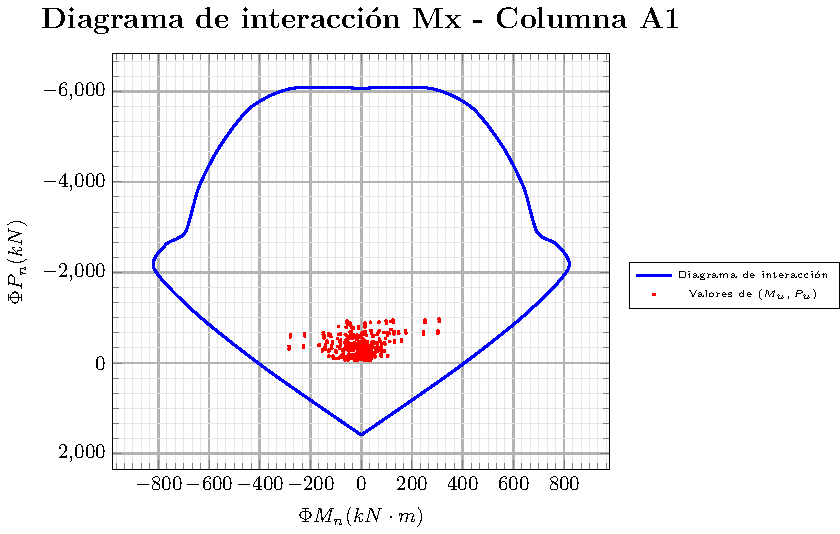
\includegraphics[width=\textwidth]{images/COLUMNAS/C_A1_MX.pdf}
         \caption{Diagrama de interacción en dirección X}
         \label{fig:CA1 X}
     \end{subfigure}
     \hfill
     \begin{subfigure}[b]{0.45\textwidth}
         \centering
         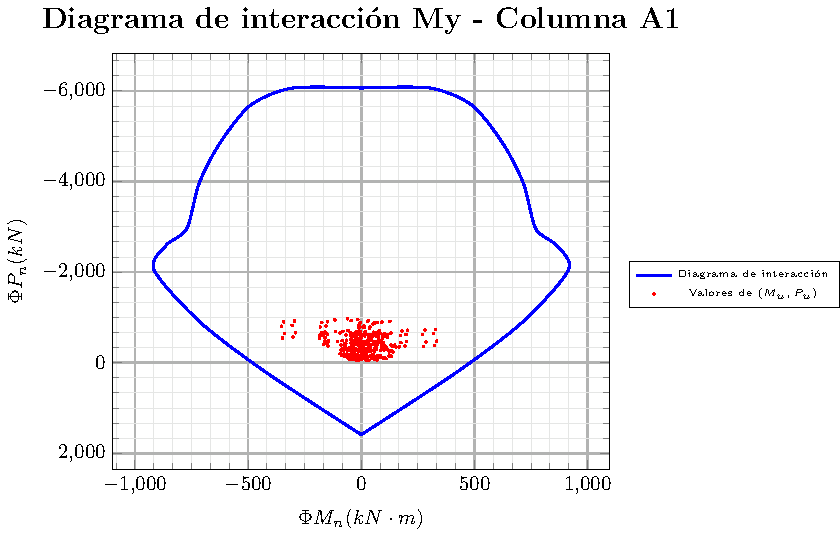
\includegraphics[width=\textwidth]{images/COLUMNAS/C_A1_MY.pdf}
         \caption{Diagrama de interacción en dirección Y}
         \label{fig:CA1 Y}
     \end{subfigure}
    
        \caption{Diagramas de interacción para la columna A1}
        \label{fig:A1}
\end{figure}

%%% COLUMNA A2--------------------------------

\begin{figure}[H]
     \centering
     \begin{subfigure}[b]{0.45\textwidth}
         \centering
         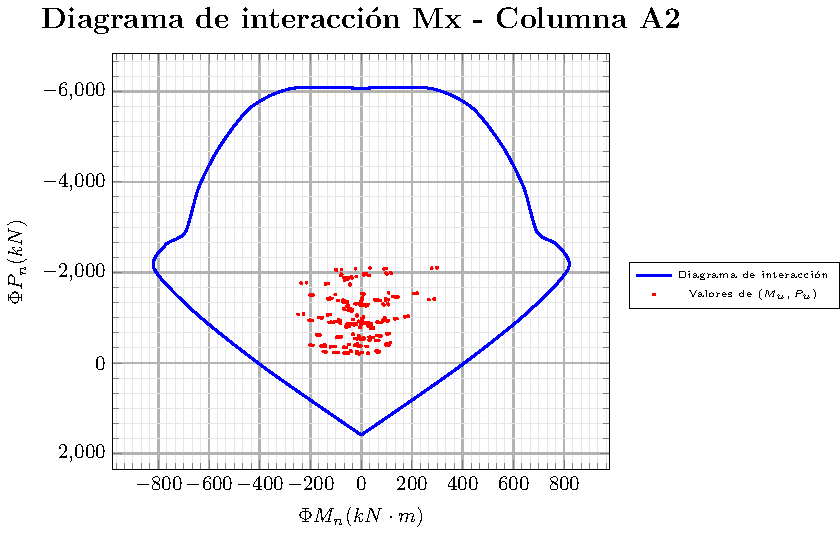
\includegraphics[width=\textwidth]{images/COLUMNAS/C_A2_MX.pdf}
         \caption{Diagrama de interacción en dirección X}
         \label{fig:CA2 X}
     \end{subfigure}
     \hfill
     \begin{subfigure}[b]{0.45\textwidth}
         \centering
         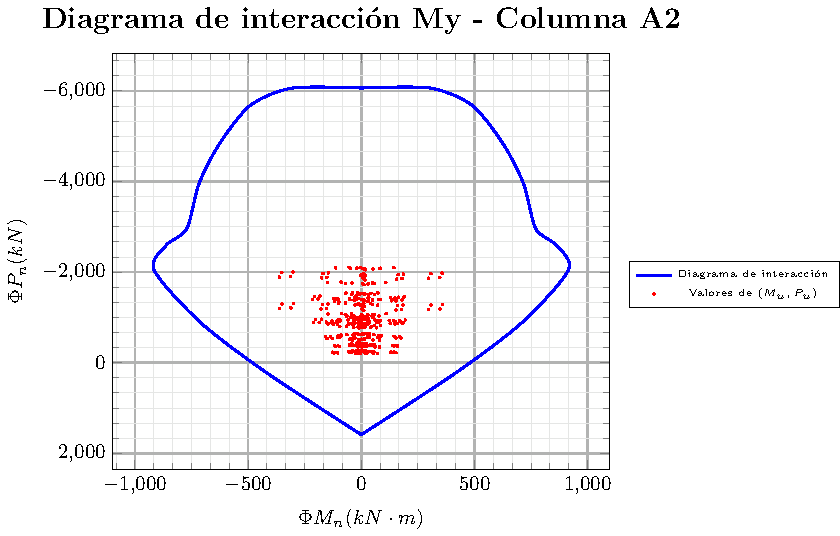
\includegraphics[width=\textwidth]{images/COLUMNAS/C_A2_MY_.pdf}
         \caption{Diagrama de interacción en dirección Y}
         \label{fig:CA2 Y}
     \end{subfigure}
    
        \caption{Diagramas de interacción para la columna A2}
        \label{fig:A2}
\end{figure}

%%% COLUMNA A3--------------------------------

\begin{figure}[H]
     \centering
     \begin{subfigure}[b]{0.45\textwidth}
         \centering
         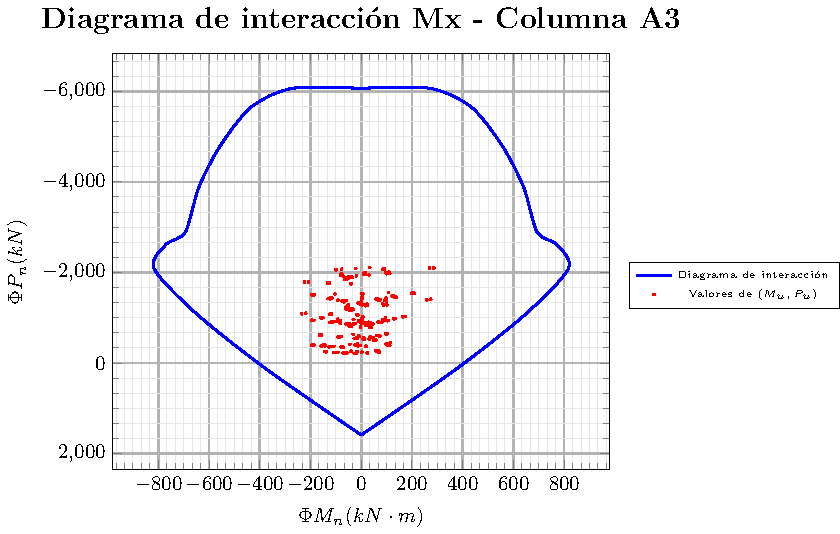
\includegraphics[width=\textwidth]{images/COLUMNAS/C_A3_MX_.pdf}
         \caption{Diagrama de interacción en dirección X}
         \label{fig:CA3 X}
     \end{subfigure}
     \hfill
     \begin{subfigure}[b]{0.45\textwidth}
         \centering
         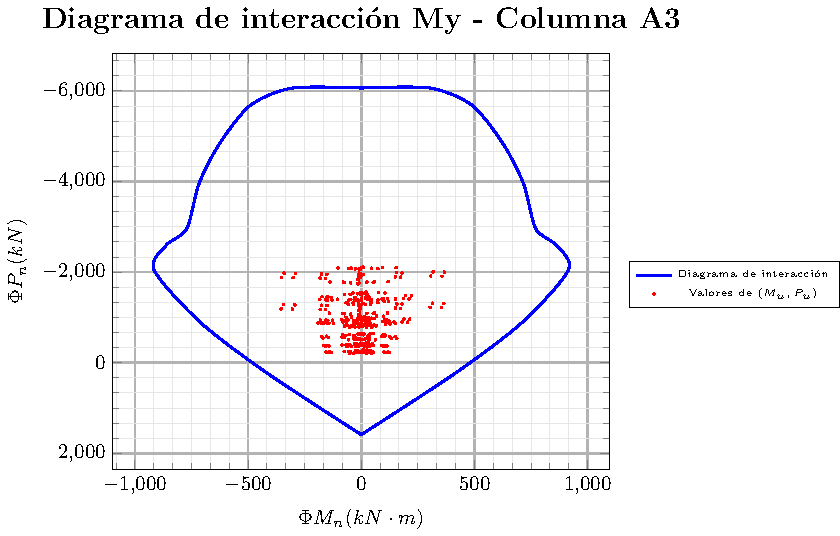
\includegraphics[width=\textwidth]{images/COLUMNAS/C_A3_MY__.pdf}
         \caption{Diagrama de interacción en dirección Y}
         \label{fig:CA3 Y}
     \end{subfigure}
    
        \caption{Diagramas de interacción para la columna A3}
        \label{fig:A3}
\end{figure}

%%% COLUMNA A4--------------------------------

\begin{figure}[H]
     \centering
     \begin{subfigure}[b]{0.45\textwidth}
         \centering
         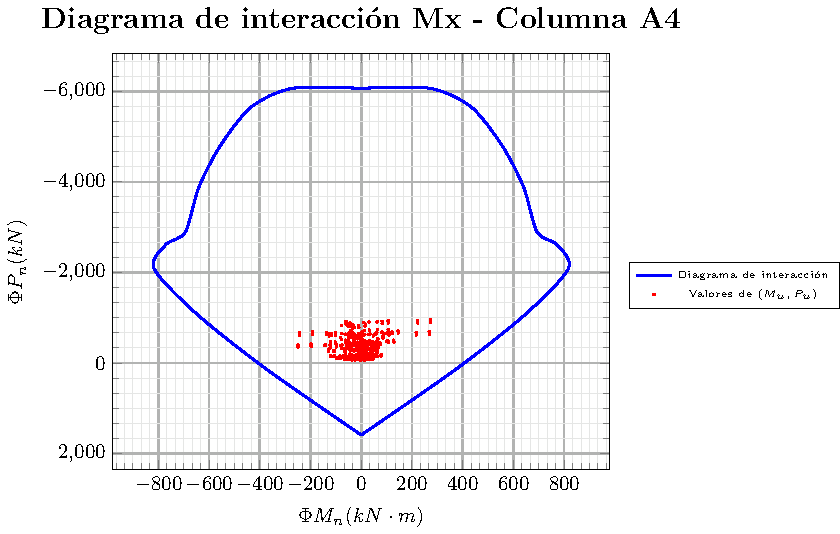
\includegraphics[width=\textwidth]{images/COLUMNAS/C_A4_MX__.pdf}
         \caption{Diagrama de interacción en dirección X}
         \label{fig:CA4 X}
     \end{subfigure}
     \hfill
     \begin{subfigure}[b]{0.45\textwidth}
         \centering
         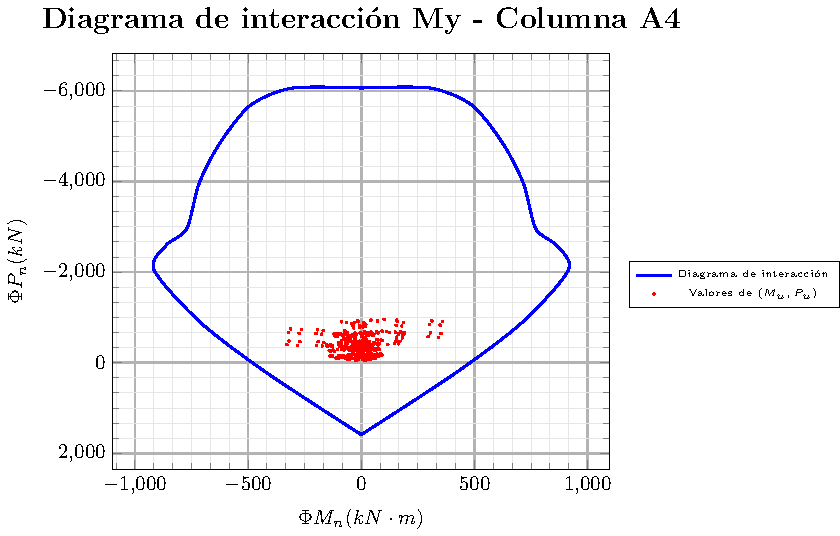
\includegraphics[width=\textwidth]{images/COLUMNAS/C_A4_MY__.pdf}
         \caption{Diagrama de interacción en dirección Y}
         \label{fig:CA4 Y}
     \end{subfigure}
    
        \caption{Diagramas de interacción para la columna A4}
        \label{fig:A4}
\end{figure}

%%% COLUMNA B1--------------------------------

\begin{figure}[H]
     \centering
     \begin{subfigure}[b]{0.45\textwidth}
         \centering
         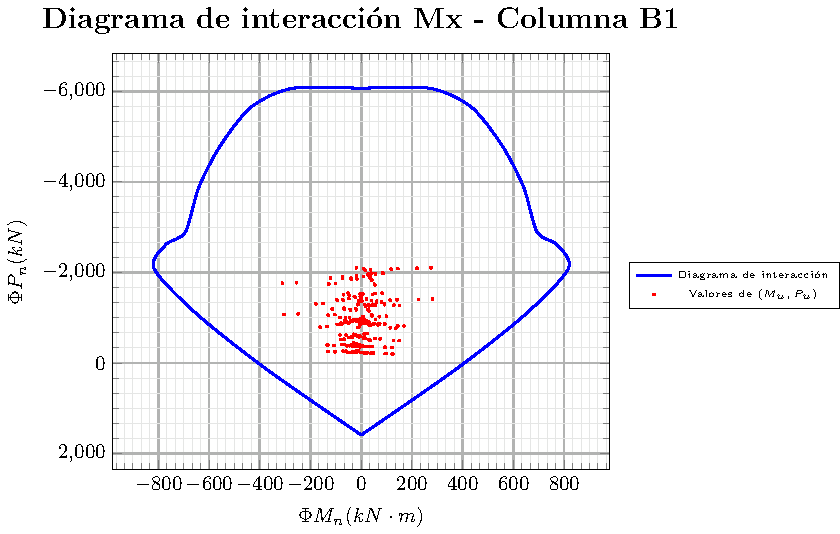
\includegraphics[width=\textwidth]{images/COLUMNAS/C_B1_MX.pdf}
         \caption{Diagrama de interacción en dirección X}
         \label{fig:CB1 X}
     \end{subfigure}
     \hfill
     \begin{subfigure}[b]{0.45\textwidth}
         \centering
         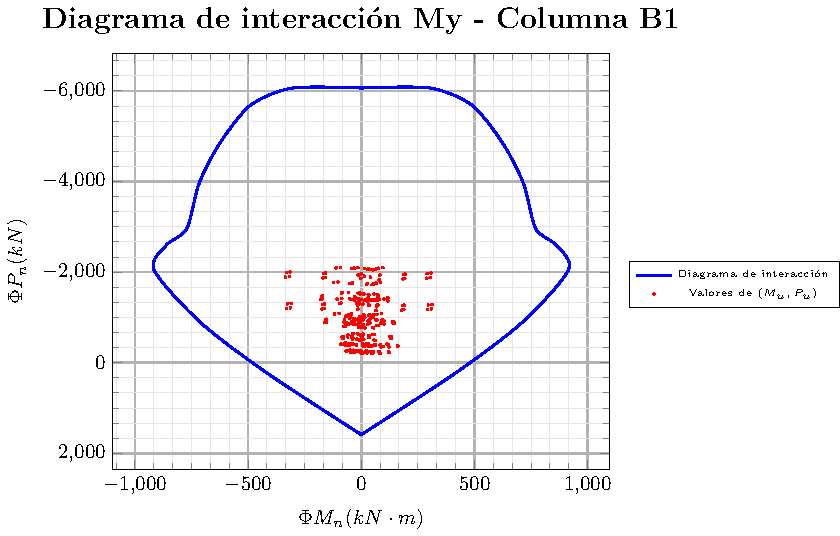
\includegraphics[width=\textwidth]{images/COLUMNAS/C_B1_MY_.pdf}
         \caption{Diagrama de interacción en dirección Y}
         \label{fig:CB1 Y}
     \end{subfigure}
    
        \caption{Diagramas de interacción para la columna B1}
        \label{fig:B1}
\end{figure}

%%% COLUMNA B2--------------------------------

\begin{figure}[H]
     \centering
     \begin{subfigure}[b]{0.45\textwidth}
         \centering
         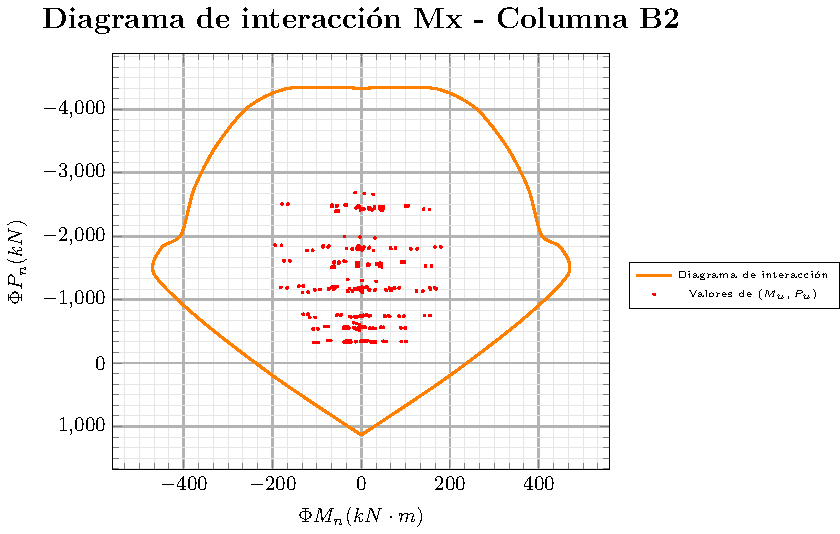
\includegraphics[width=\textwidth]{images/COLUMNAS/C_B2_MX.pdf}
         \caption{Diagrama de interacción en dirección X}
         \label{fig:CB2 X}
     \end{subfigure}
     \hfill
     \begin{subfigure}[b]{0.45\textwidth}
         \centering
         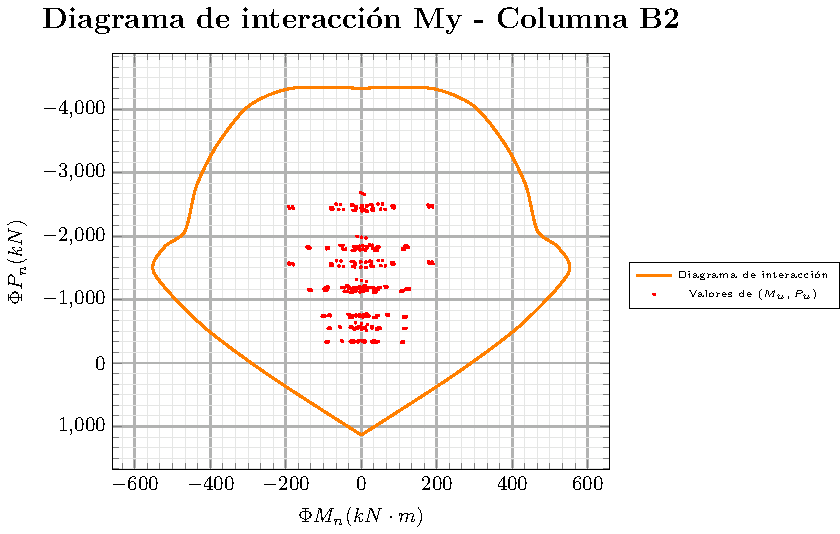
\includegraphics[width=\textwidth]{images/COLUMNAS/C_B2_MY.pdf}
         \caption{Diagrama de interacción en dirección Y}
         \label{fig:CB2 Y}
     \end{subfigure}
    
        \caption{Diagramas de interacción para la columna B2}
        \label{fig:B2}
\end{figure}

%%% COLUMNA B3--------------------------------

\begin{figure}[H]
     \centering
     \begin{subfigure}[b]{0.45\textwidth}
         \centering
         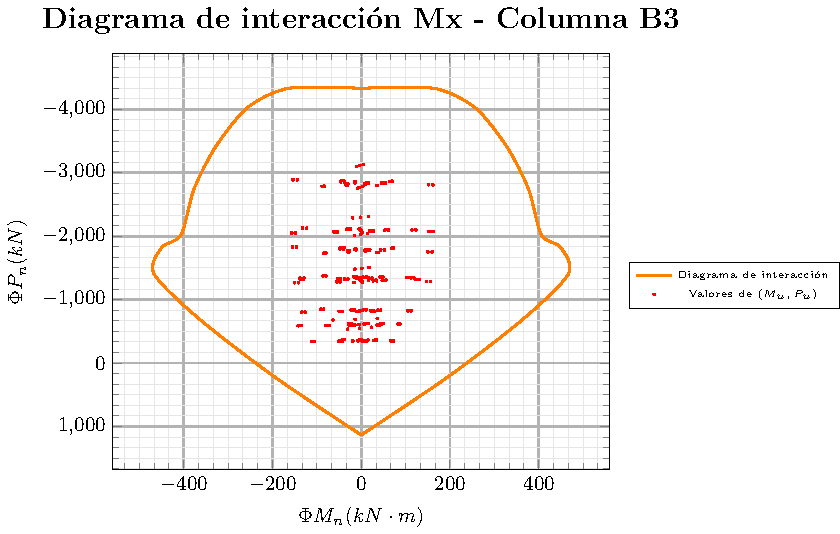
\includegraphics[width=\textwidth]{images/COLUMNAS/C_B3_MX_.pdf}
         \caption{Diagrama de interacción en dirección X}
         \label{fig:CB3 X}
     \end{subfigure}
     \hfill
     \begin{subfigure}[b]{0.45\textwidth}
         \centering
         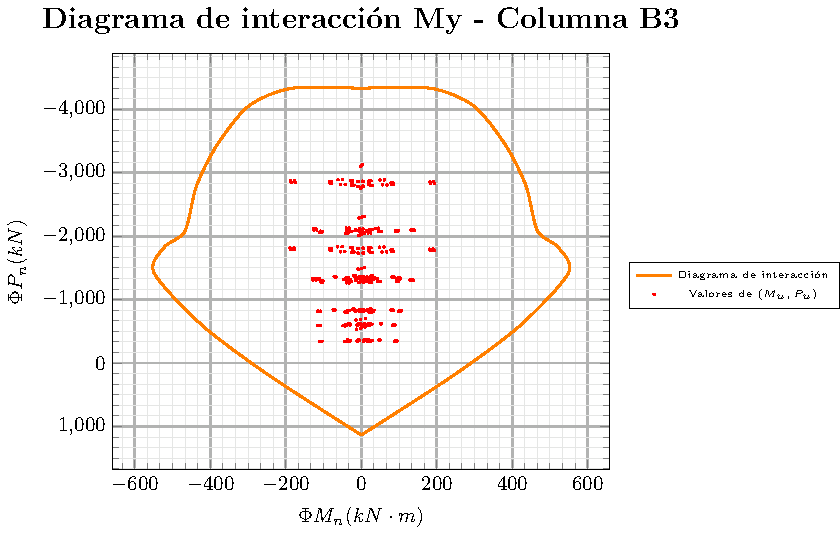
\includegraphics[width=\textwidth]{images/COLUMNAS/C_B3_MY_.pdf}
         \caption{Diagrama de interacción en dirección Y}
         \label{fig:CB3 Y}
     \end{subfigure}
    
        \caption{Diagramas de interacción para la columna B3}
        \label{fig:B3}
\end{figure}

%%% COLUMNA B4--------------------------------

\begin{figure}[H]
     \centering
     \begin{subfigure}[b]{0.45\textwidth}
         \centering
         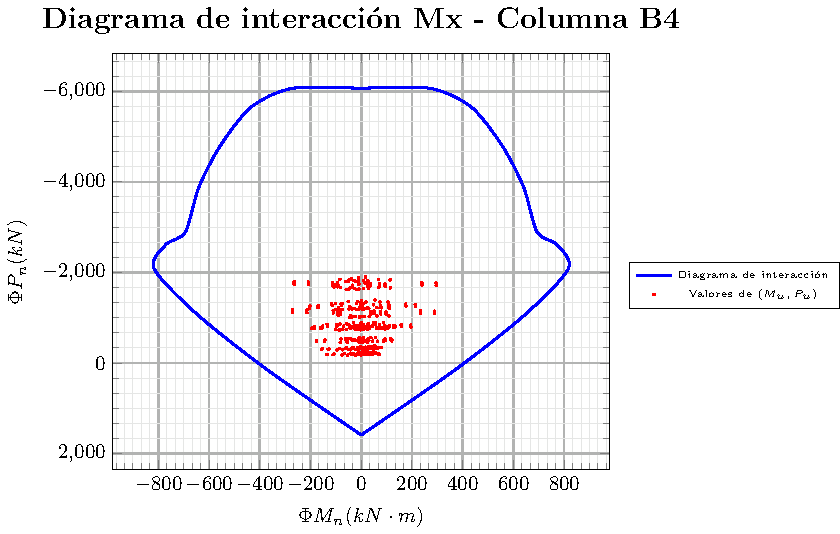
\includegraphics[width=\textwidth]{images/COLUMNAS/C_B4_MX_.pdf}
         \caption{Diagrama de interacción en dirección X}
         \label{fig:CB4 X}
     \end{subfigure}
     \hfill
     \begin{subfigure}[b]{0.45\textwidth}
         \centering
         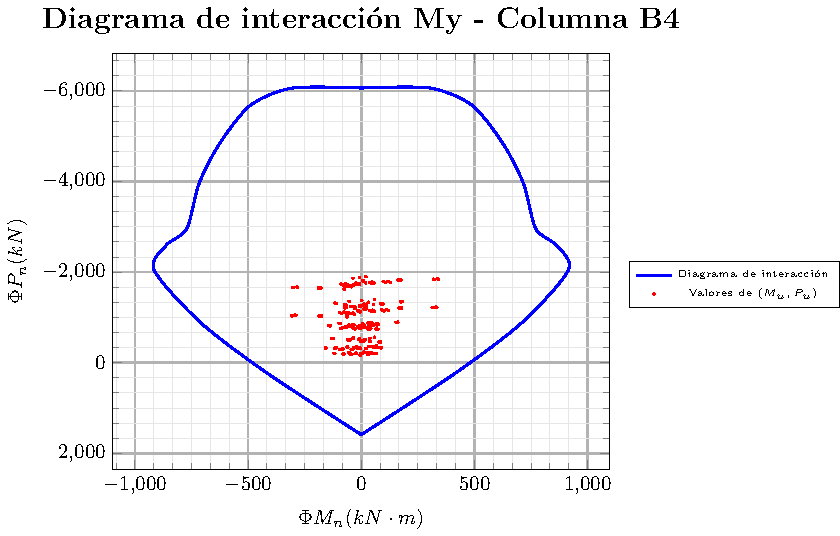
\includegraphics[width=\textwidth]{images/COLUMNAS/C_B4_MY__.pdf}
         \caption{Diagrama de interacción en dirección Y}
         \label{fig:CB4 Y}
     \end{subfigure}
    
        \caption{Diagramas de interacción para la columna B4}
        \label{fig:B4}
\end{figure}

%%% COLUMNA C1--------------------------------

\begin{figure}[H]
     \centering
     \begin{subfigure}[b]{0.45\textwidth}
         \centering
         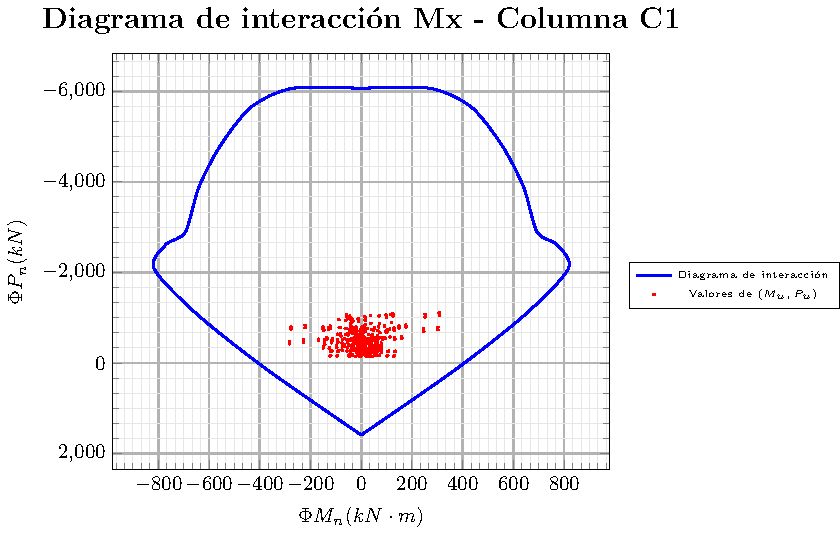
\includegraphics[width=\textwidth]{images/COLUMNAS/C_C1_MX_.pdf}
         \caption{Diagrama de interacción en dirección X}
         \label{fig:CC1 X}
     \end{subfigure}
     \hfill
     \begin{subfigure}[b]{0.45\textwidth}
         \centering
         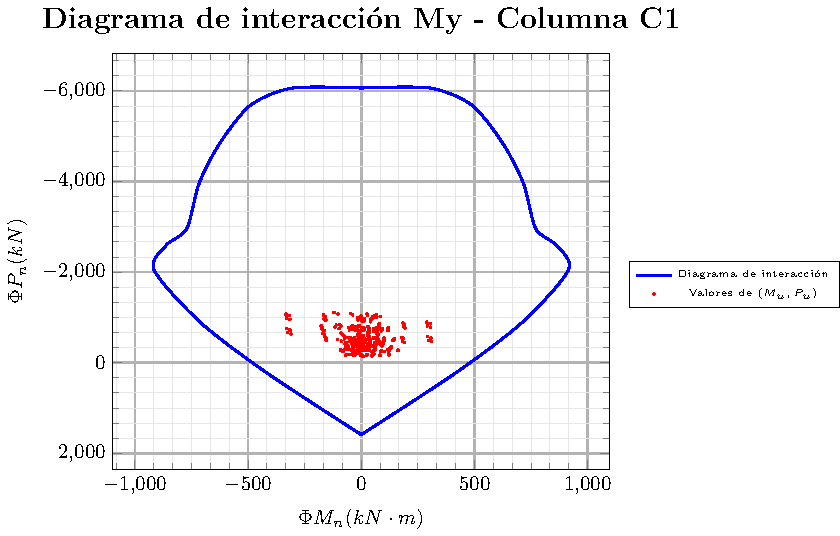
\includegraphics[width=\textwidth]{images/COLUMNAS/C_C1_MY__.pdf}
         \caption{Diagrama de interacción en dirección Y}
         \label{fig:CC1 Y}
     \end{subfigure}
    
        \caption{Diagramas de interacción para la columna C1}
        \label{fig:C1}
\end{figure}

%%% COLUMNA C2--------------------------------

\begin{figure}[H]
     \centering
     \begin{subfigure}[b]{0.45\textwidth}
         \centering
         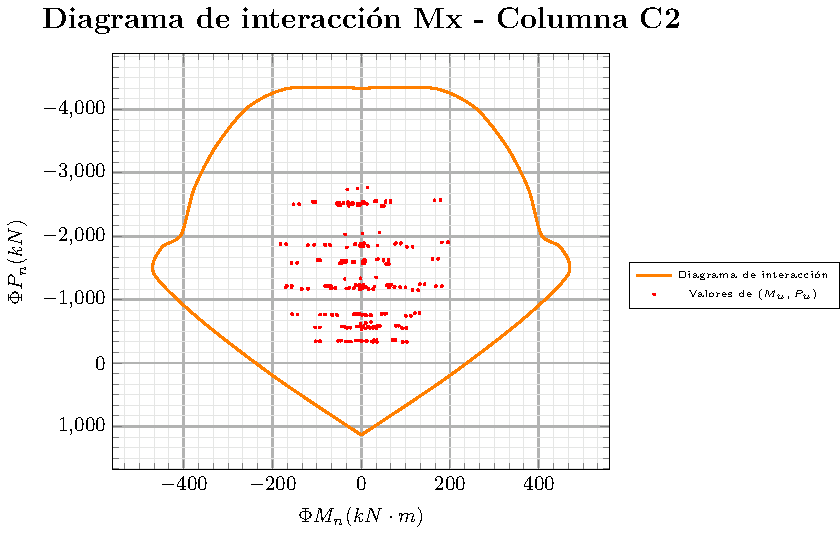
\includegraphics[width=\textwidth]{images/COLUMNAS/C_C2_MX_.pdf}
         \caption{Diagrama de interacción en dirección X}
         \label{fig:CC2 X}
     \end{subfigure}
     \hfill
     \begin{subfigure}[b]{0.45\textwidth}
         \centering
         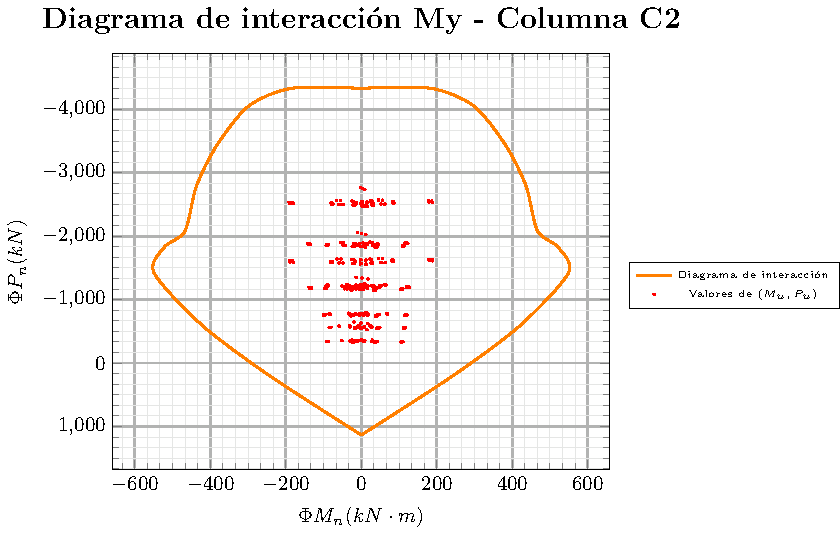
\includegraphics[width=\textwidth]{images/COLUMNAS/C_C2_MY.pdf}
         \caption{Diagrama de interacción en dirección Y}
         \label{fig:CC2 Y}
     \end{subfigure}
    
        \caption{Diagramas de interacción para la columna C2}
        \label{fig:C2}
\end{figure}

%%% COLUMNA C3--------------------------------

\begin{figure}[H]
     \centering
     \begin{subfigure}[b]{0.45\textwidth}
         \centering
         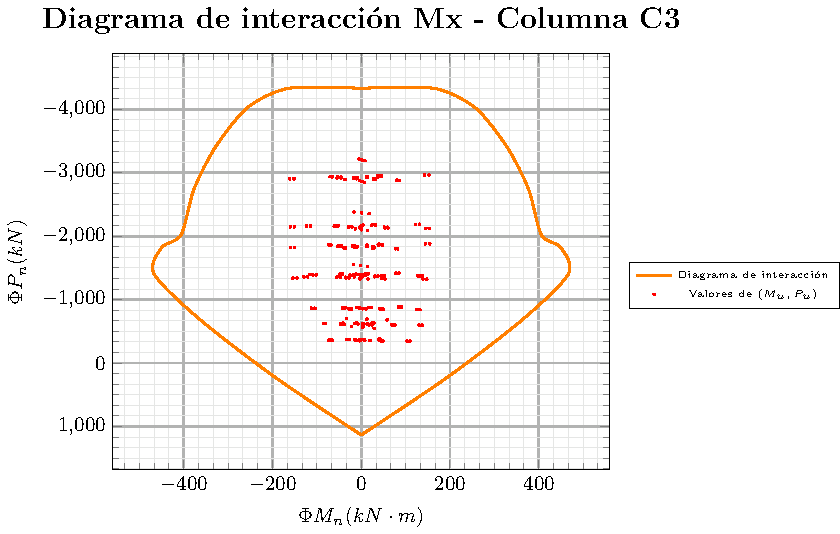
\includegraphics[width=\textwidth]{images/COLUMNAS/C_C3_MX__.pdf}
         \caption{Diagrama de interacción en dirección X}
         \label{fig:CC3 X}
     \end{subfigure}
     \hfill
     \begin{subfigure}[b]{0.45\textwidth}
         \centering
         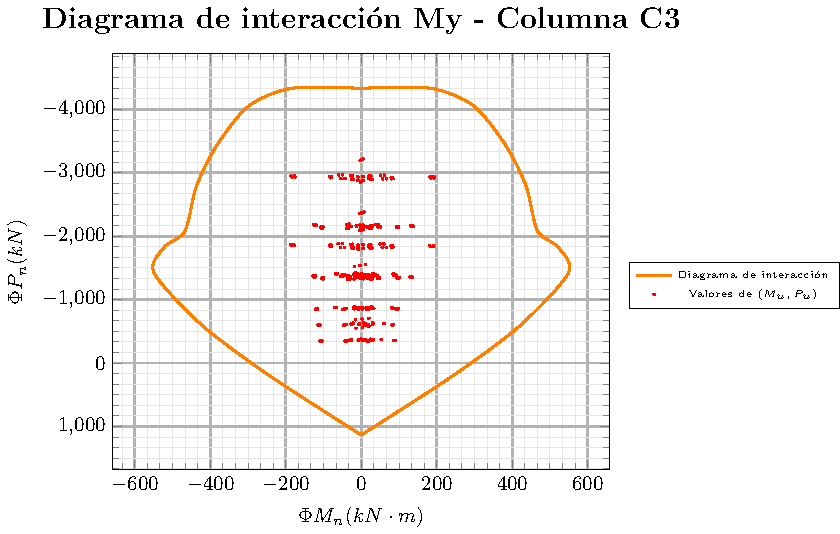
\includegraphics[width=\textwidth]{images/COLUMNAS/C_C3_MY__.pdf}
         \caption{Diagrama de interacción en dirección Y}
         \label{fig:CC3 Y}
     \end{subfigure}
    
        \caption{Diagramas de interacción para la columna C3}
        \label{fig:C3}
\end{figure}

%%% COLUMNA C4--------------------------------

\begin{figure}[H]
     \centering
     \begin{subfigure}[b]{0.45\textwidth}
         \centering
         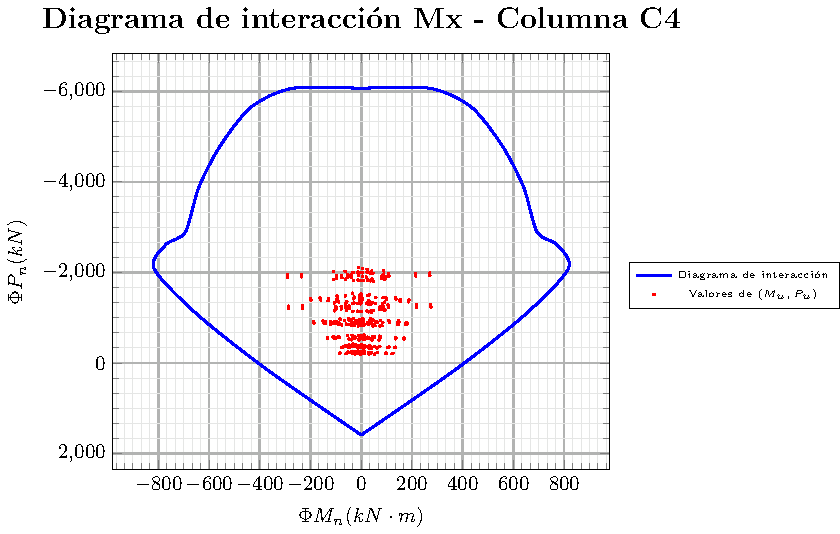
\includegraphics[width=\textwidth]{images/COLUMNAS/C_C4_MX__.pdf}
         \caption{Diagrama de interacción en dirección X}
         \label{fig:CC4 X}
     \end{subfigure}
     \hfill
     \begin{subfigure}[b]{0.45\textwidth}
         \centering
         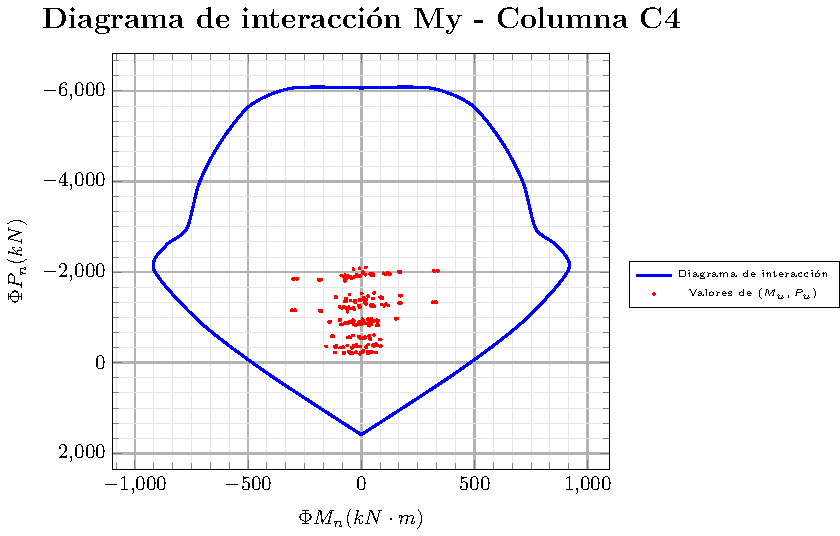
\includegraphics[width=\textwidth]{images/COLUMNAS/C_C4_MY___.pdf}
         \caption{Diagrama de interacción en dirección Y}
         \label{fig:CC4 Y}
     \end{subfigure}
    
        \caption{Diagramas de interacción para la columna C4}
        \label{fig:C4}
\end{figure}

%%% COLUMNA D1--------------------------------

\begin{figure}[H]
     \centering
     \begin{subfigure}[b]{0.45\textwidth}
         \centering
         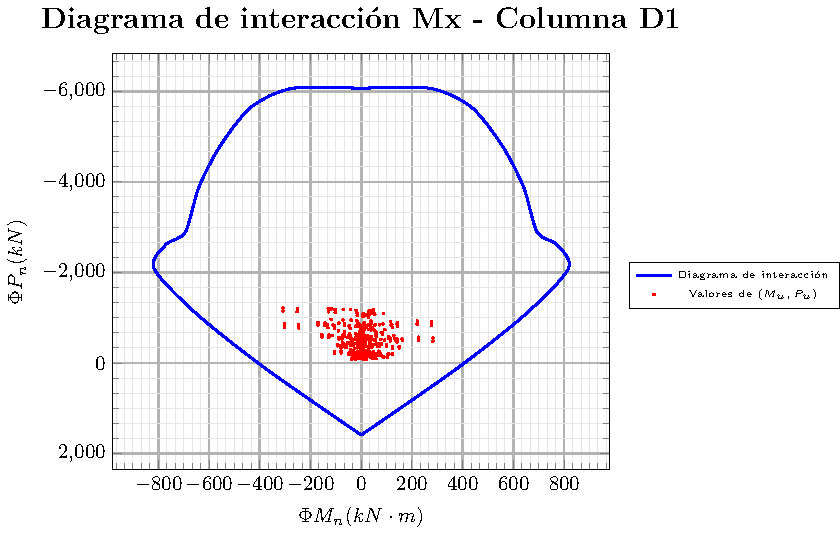
\includegraphics[width=\textwidth]{images/COLUMNAS/C_D1_MX.pdf}
         \caption{Diagrama de interacción en dirección X}
         \label{fig:CD1 X}
     \end{subfigure}
     \hfill
     \begin{subfigure}[b]{0.45\textwidth}
         \centering
         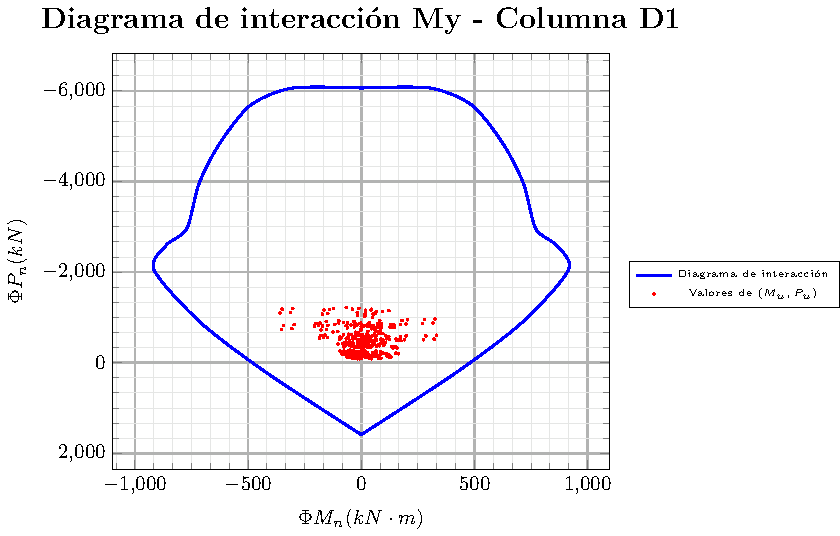
\includegraphics[width=\textwidth]{images/COLUMNAS/C_D1_MY_.pdf}
         \caption{Diagrama de interacción en dirección Y}
         \label{fig:CD1 Y}
     \end{subfigure}
    
        \caption{Diagramas de interacción para la columna D1}
        \label{fig:D1}
\end{figure}

%%% COLUMNA D2--------------------------------

\begin{figure}[H]
     \centering
     \begin{subfigure}[b]{0.45\textwidth}
         \centering
         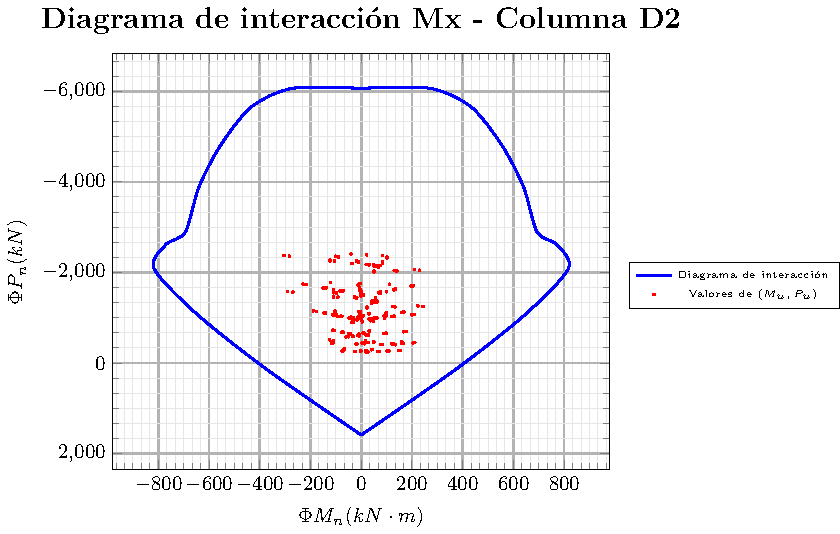
\includegraphics[width=\textwidth]{images/COLUMNAS/C_D2_MX_.pdf}
         \caption{Diagrama de interacción en dirección X}
         \label{fig:CD2 X}
     \end{subfigure}
     \hfill
     \begin{subfigure}[b]{0.45\textwidth}
         \centering
         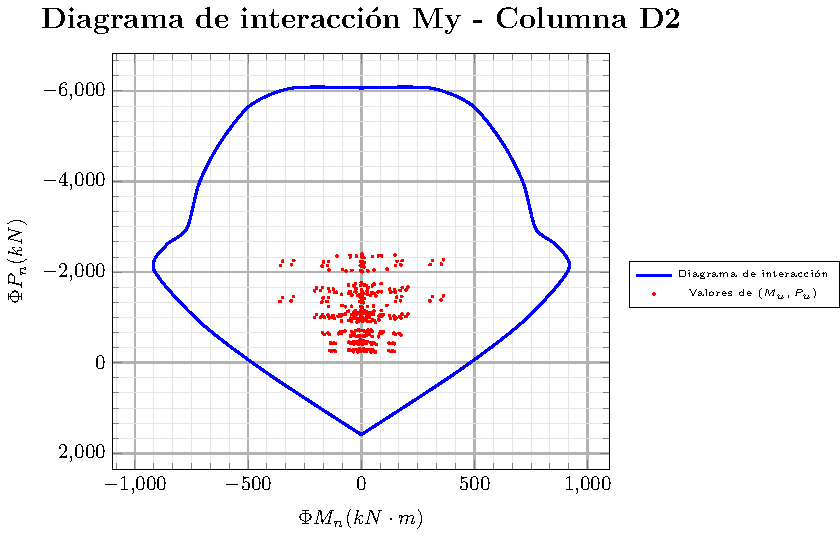
\includegraphics[width=\textwidth]{images/COLUMNAS/C_D2_MY__.pdf}
         \caption{Diagrama de interacción en dirección Y}
         \label{fig:CD2 Y}
     \end{subfigure}
    
        \caption{Diagramas de interacción para la columna D2}
        \label{fig:D2}
\end{figure}

%%% COLUMNA D3--------------------------------

\begin{figure}[H]
     \centering
     \begin{subfigure}[b]{0.45\textwidth}
         \centering
         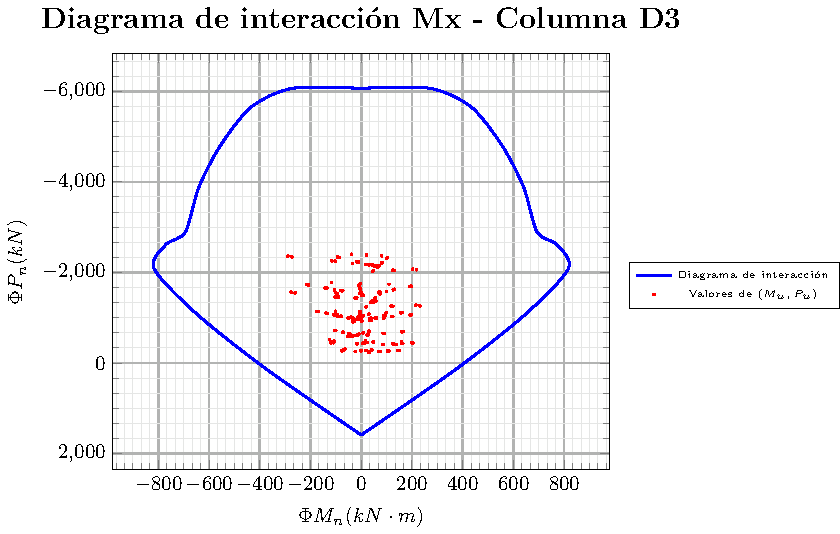
\includegraphics[width=\textwidth]{images/COLUMNAS/C_D3_MX__.pdf}
         \caption{Diagrama de interacción en dirección X}
         \label{fig:CD3 X}
     \end{subfigure}
     \hfill
     \begin{subfigure}[b]{0.45\textwidth}
         \centering
         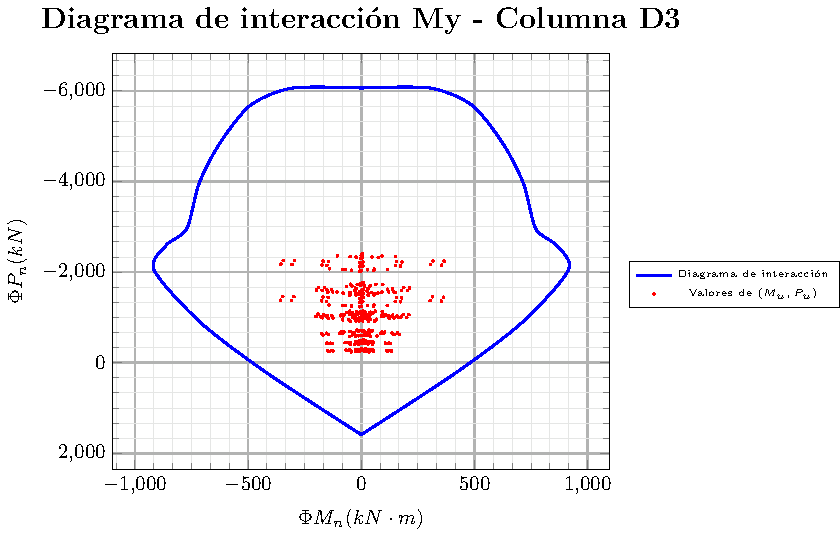
\includegraphics[width=\textwidth]{images/COLUMNAS/C_D3_MY___.pdf}
         \caption{Diagrama de interacción en dirección Y}
         \label{fig:CD3 Y}
     \end{subfigure}
    
        \caption{Diagramas de interacción para la columna D3}
        \label{fig:D3}
\end{figure}

%%% COLUMNA D4--------------------------------

\begin{figure}[H]
     \centering
     \begin{subfigure}[b]{0.45\textwidth}
         \centering
         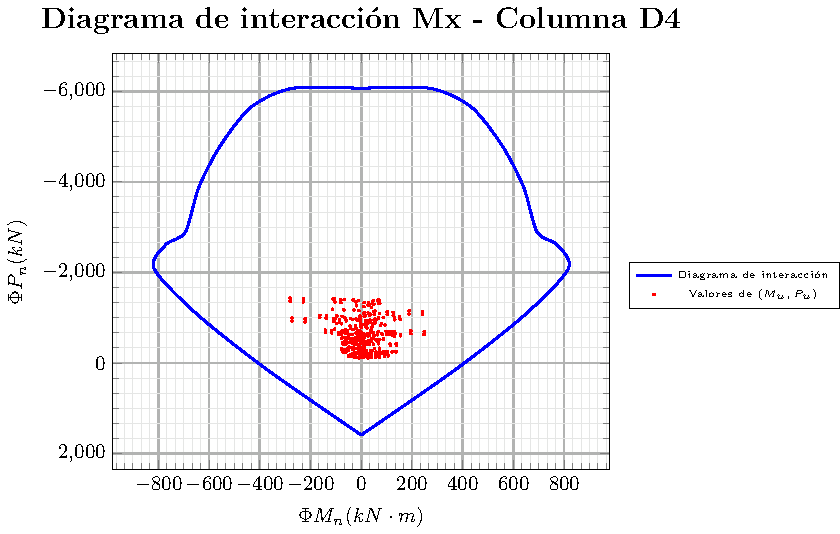
\includegraphics[width=\textwidth]{images/COLUMNAS/C_D4_MX___.pdf}
         \caption{Diagrama de interacción en dirección X}
         \label{fig:CD4 X}
     \end{subfigure}
     \hfill
     \begin{subfigure}[b]{0.45\textwidth}
         \centering
         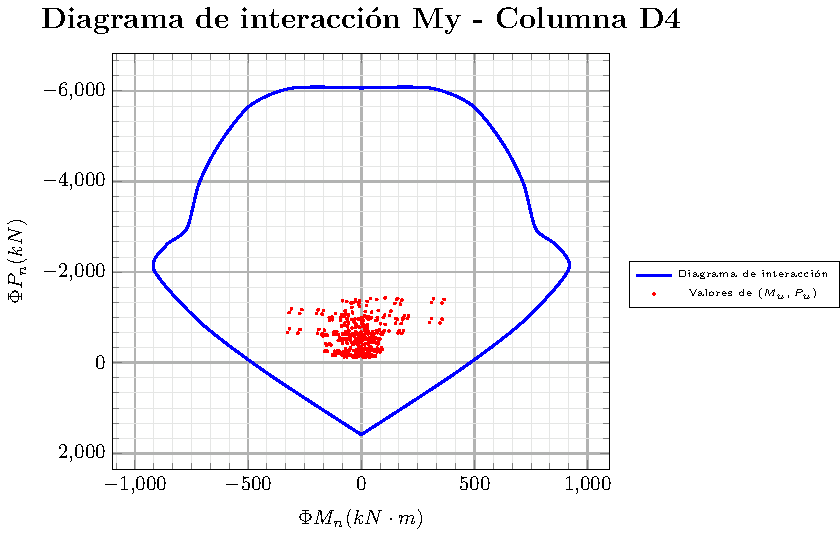
\includegraphics[width=\textwidth]{images/COLUMNAS/C_D4_MY__.pdf}
         \caption{Diagrama de interacción en dirección Y}
         \label{fig:CD4 Y}
     \end{subfigure}
    
        \caption{Diagramas de interacción para la columna D4}
        \label{fig:D4}
\end{figure}






